% Chapter 1

\chapter[Introduction]{Introduction} % Main chapter title

\label{Chapter1} % For referencing the chapter elsewhere, use \ref{Chapter1} 

%----------------------------------------------------------------------------------------

% Define some commands to keep the formatting separated from the content 
\newcommand{\keyword}[1]{\textbf{#1}}
\newcommand{\tabhead}[1]{\textbf{#1}}
\newcommand{\code}[1]{\texttt{#1}}
\newcommand{\file}[1]{\texttt{\bfseries#1}}
\newcommand{\option}[1]{\texttt{\itshape#1}}

%----------------------------------------------------------------------------------------

\section{Background}
Recent years have seen rapid development in robotics technology due to the constantly increasing availability of computing power, reductions in the cost of hardware such as digital sensors and actuators, and developments in the application of artificial intelligence to robot control. This has lead to robots being used to perform increasingly complex tasks and solve ever more difficult problems. Many new areas of robotics research have emerged as a result, as researchers strive to find new and better ways to apply this technology, entering into problem domains once thought to be impossible for robots. Whole new robotics paradigms have been created as the standard model of a single, complex, expensive robot has been questioned, opening the door for cooperative robots, multi-robot systems, and more specifically swarm robotics.

Studies into the self-organising behaviour of social insect colonies, and the development of mathematical models based on these behaviours, led to the development of a field of research referred to as Swarm Intelligence (SI). The aim of these models is to determine how large numbers of individual agents are able to solve problems collectively, with each agent using only local information, and without any centralised control. Swarm Robotics developed from a desire to apply these concepts in practice to real world problem solving. Dorigo et al. describe swarm robotics as `\textit{the study of how to design groups of robots that operate without relying on any external infrastructure or on any form of centralised control ... }[where]\textit{ the collective behaviour of the robots results from local interactions between the robots and between the robots and the environment}\cite{Dorigo:2014}'. Swarm robotics has since emerged as a promising area of research for solving problems which would be infeasibly difficult or expensive for a conventional robotics approach.

%----------------------------------------------------------------------------------------

\section{Project Context} \label{ProjectContext}
Developing and debugging robotics behaviours has always been a challenging task. Whilst traditional software is run in a purely digital environment with a tightly controlled set of inputs and outputs to and from the physical world, robots must interact constantly with the physical world in order to satisfy their intended purpose. Robots are therefore subject to a much wider array of inputs and outputs, and to a huge number of changing variables within their environment at any given time. Often these variables and inputs are continuous in nature, rather than the discreet inputs more commonly used by traditional computers. This makes detecting, reproducing and correcting specific bugs in a robot's behaviour significantly harder than in traditional software. A large number of continuous inputs leads to a theoretically infinite set of possible input configurations, and can therefore make reproducing the exact conditions under which a bug occurred extremely difficult if not impossible. 

Another of the main difficulties comes from the layers of abstraction between the real world, the robot, and the human developer. There is a potential disconnect between the robot's interpretation of the world and the reality of the world itself. Inaccuracies in this interpretation can be caused by any number of issues, including sensor hardware problems as well as software bugs. This can cause erroneous behaviour that might be wrongly attributed to a bug in the robot's behavioural code or decision making, rather than its perception. This issue can be compounded by the fact that the human operator's knowledge of the robot's interpretation of the world might also be inaccurate or incomplete. Figure \ref{fig:DebuggingInformation} shows these different layers of information abstraction when dealing with a robotic system. The arrow highlighted in red shows where many of these abstraction related debugging difficulties occur. Retrieving human readable information from a robot in a timely manner whilst it is running is often non-trivial, and what the robot sees and what the human operator thinks the robot sees may differ significantly.

\begin{figure}
	\centering
	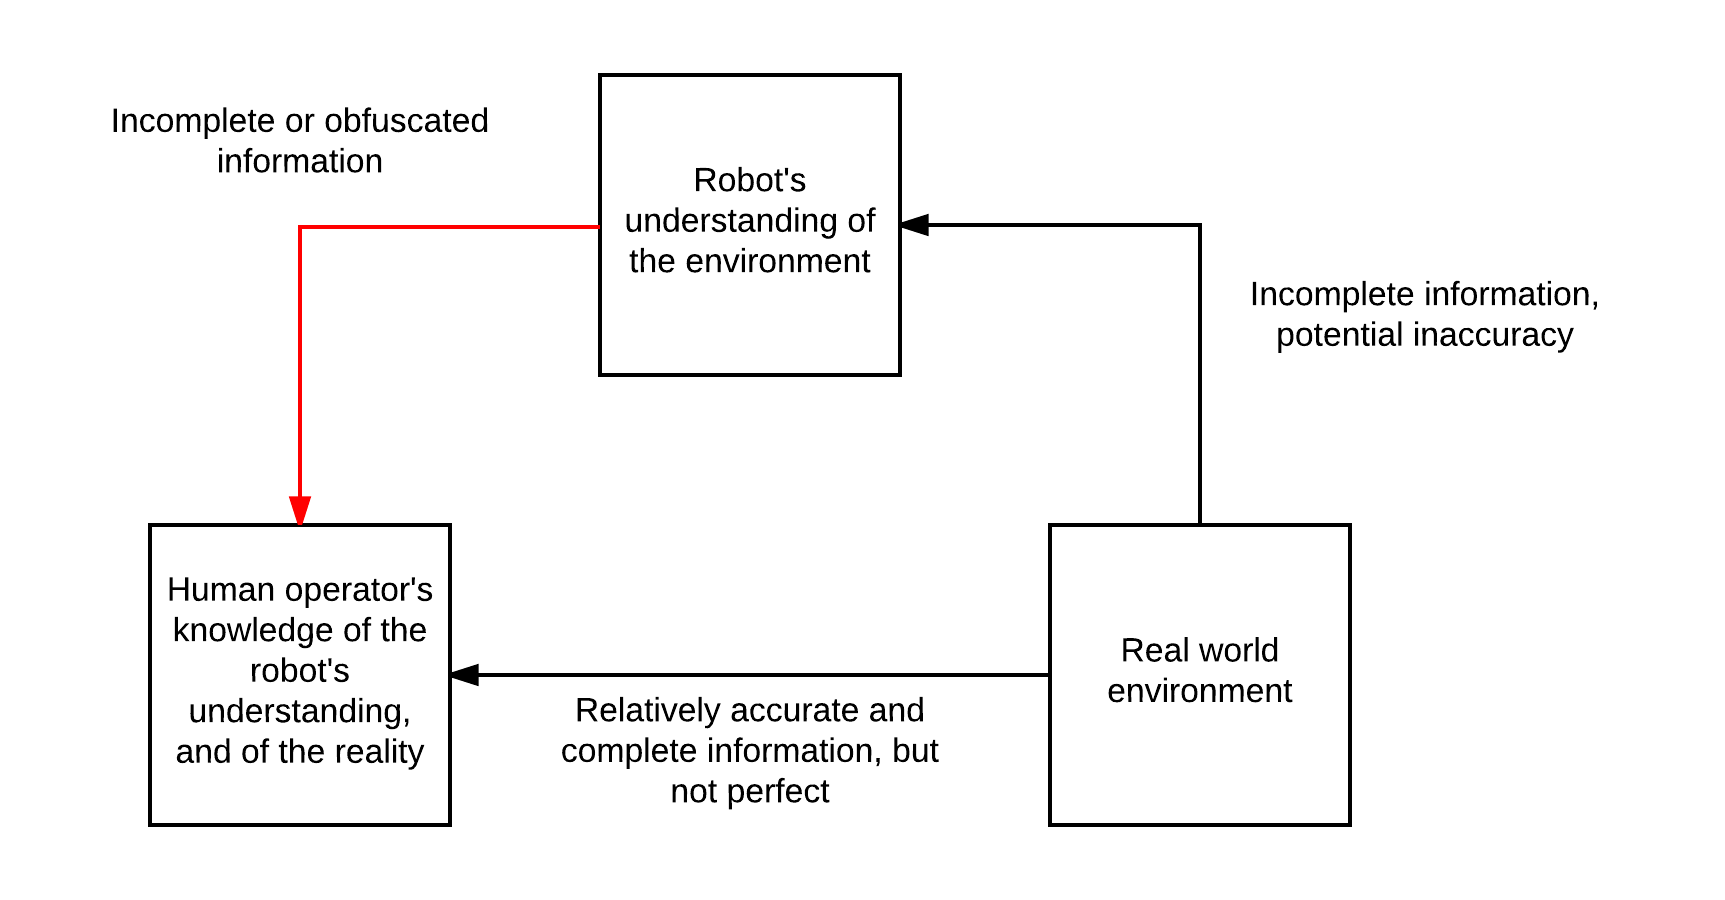
\includegraphics{Figures/RobotDebuggingInformationAbstraction.png}
	\decoRule
	\caption[Debugging information abstraction diagram]{Layers of information abstraction in robotics debugging.}
	\label{fig:DebuggingInformation}
\end{figure}

This problem is made significantly more complex when working with multi-robot systems, and especially swarm robotics. Introducing multiple robots multiplies the number of potential variables and increases the amount of information required to describe the system, hence both the number of points where a bug may be occurring and the amount of information the operator needs in order to locate it are also increased. The decentralised nature of swarm robotics systems further exacerbates this problem through the lack of a single, central control point, where information for the whole system can be retrieved.

Traditional software debugging tools are predominantly text based, and often require that program execution is paused in order to examine internal values. These tool are therefore often insufficient for robotics applications, as the quantities of data produced by a robot's sensors, and used to make its decisions, can be too large and vary too rapidly for any sensible textual representation. Furthermore pausing a robots execution can be undesirable, especially if it is operating in an active real world environment. Once again swarm robotics  and multi-robot systems compound on this problem by increasing the amount of data involved, making textual representations less likely to be sufficient, and by involving multiple data sources, which traditional debugging tools are rarely designed to handle. New tools and techniques are therefore needed to retrieve data from these robotic systems and present it in a manner that allows humans to understand and process it effectively.

Virtual and augmented reality technologies have seen significant progress in the last few years, and are beginning to emerge into a large number real-world applications. Augmented reality in particular offers a promising new method for interacting with robots, and may help to overcome some of the limitations of traditional debugging tools. An augmented reality system works by capturing a view of a real world environment through a camera, and augments it with computer generated graphical elements. These graphical elements or `virtual objects' are usually positioned within the space such that they either appear to be real, physical objects, or relate to other physical objects within the space. Augmented reality systems can therefore create `hybrid-' or `mixed-reality' environments, where users are able to interact with real world objects and virtual, computer generated ones simultaneously. This shows particular promise when combined with robotics, as a mixed-reality space is one that can be shared and understood by both humans and robots. The virtual elements of an augmented reality environment are simply representations of digital data, and this data can be readily understood by a digital system such as a robot. By creating tools which effectively utilise augmented reality techniques and mixed-reality environments in conjunction with robots, it should be possible to broaden the human-robot communication channel, introducing novel ways for humans and robots to communicate and share information, with implications for all aspects of human-robot interaction. Considering debugging specifically, it is easy to imagine how converting a robot's data such as sensor readings to graphical representations, correctly positioned to reflect their spatial significance, could improve a human operator's ability to identify problems with a robot's perception and behaviour.

%----------------------------------------------------------------------------------------

\section{Project Concept} \label{ProjectConcept}
This project focuses on trying to mitigate some of the problems discussed in the previous section by improving a human operator's access to system information, thus improving the timeliness with which bugs in a swarm robotics system can be identified, located and fixed. This means designing and implementing a system capable of collecting information from multiple sources and presenting it all in one place, in a human readable manner, in real time. The information sources to be used include the individual robots themselves, as well as a live video feed of the robots and their environment. The project also attempts to incorporate ideas and techniques related to augmented reality in order to represent data retrieved from a robotic system in ways that can be more intuitively understood by a human operator than purely textual and numerical representations.

This project attempts to create a software application and associated wireless data transaction format capable of presenting a user with a single, coherent, and highly readable interface through which they can view relevant information about a swarm and it's constituent robots in real time. This includes the use of a video based tracking system to monitor robot positions, and provide the user with a view of the robots' environment. This view can then be augmented with graphical representations of relevant elements of the retrieved robot data, such as sensor readings. The robots will communicate data to the computer running the application wirelessly. The initial target robot platform is the widely used \textit{e-puck} robot \cite{epuck}, equipped with a Linux extension board and WiFi adapter. The e-puck platform is discussed in greater detail in chapter \ref{ChapterProblemAnalysis}. The diagram in figure \ref{fig:SystemArchitecture} gives a logical representation of the proposed system architecture, in terms of its component parts, including the e-puck robots, tracking camera, and the application's host computer. This report describes the design, implementation and testing of this system, and includes details of the steps undertaken to evaluate its effectiveness. Some portions of this report appeared previously in a similar form in an \textit{Initial Report} document, and are included here for completeness, with minor alterations.

\begin{figure}
	\begin{center}
	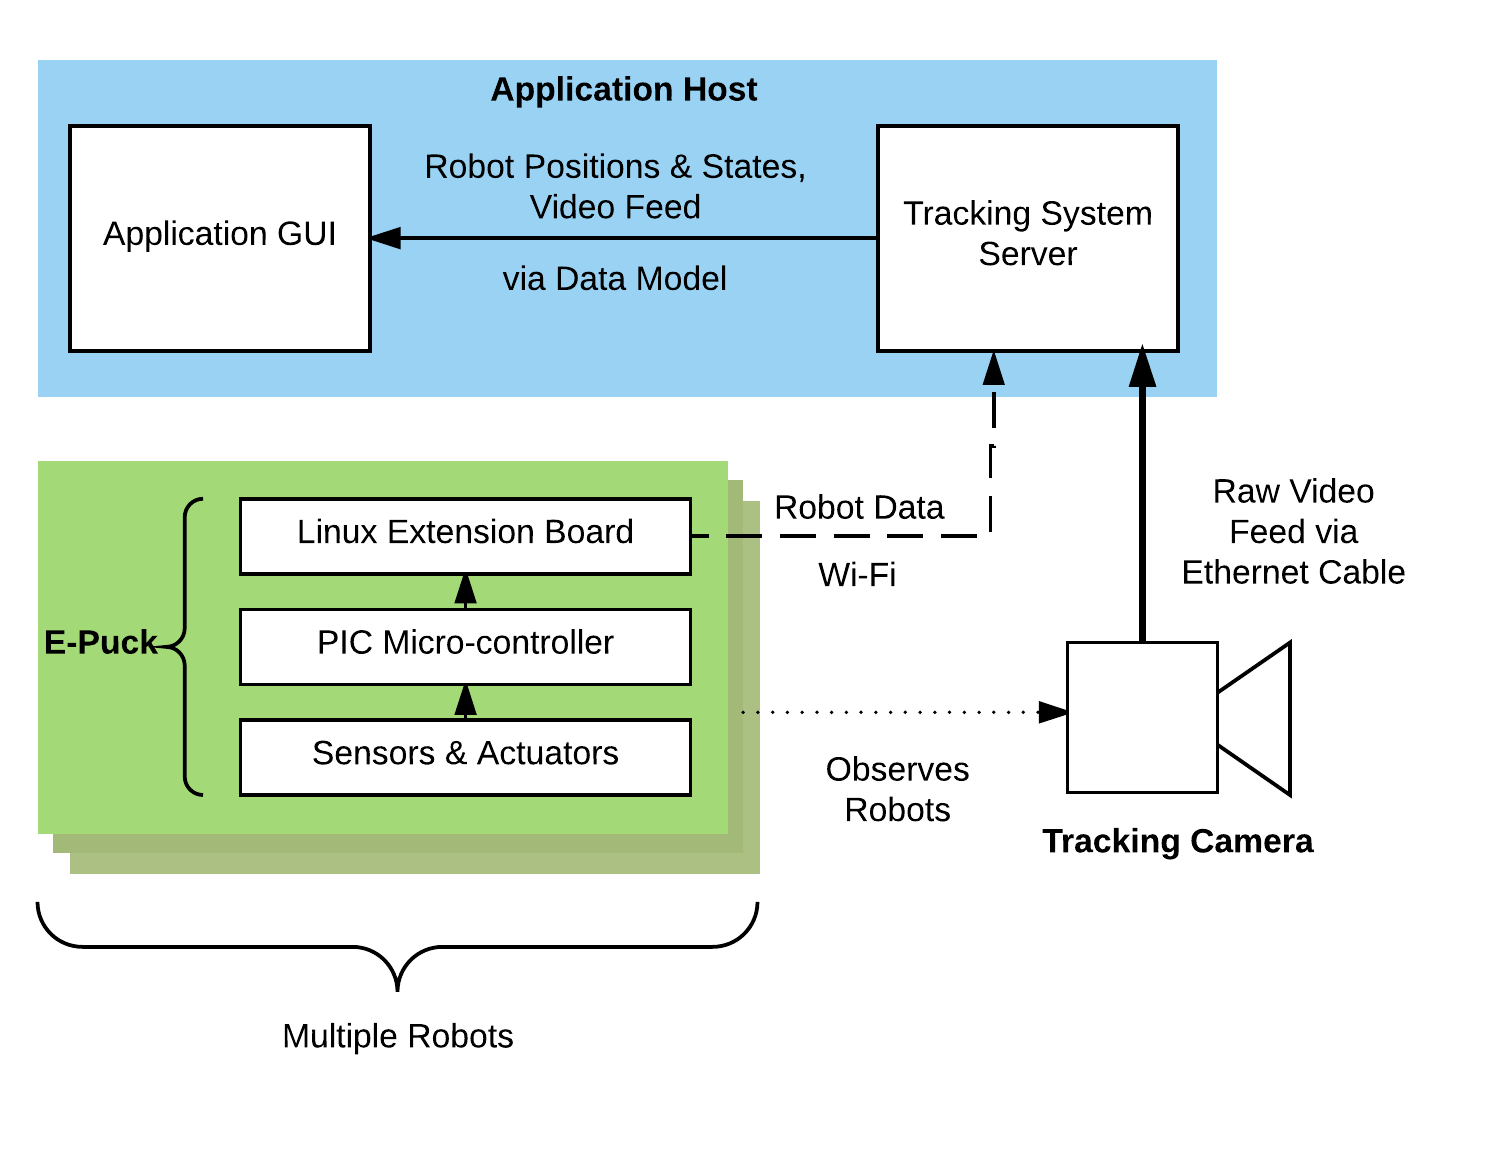
\includegraphics[scale=1]{SystemArchitecture.png}
	\decoRule
	\caption[Proposed system architecture]{The proposed system architecture.}
	\label{fig:SystemArchitecture}
	\end{center}
\end{figure}

%----------------------------------------------------------------------------------------

\section{Aim and Objectives} \label{AimAndObjectives}
Having gained an understanding of the context for this project in section \ref{ProjectContext}, and outlined the concept for the system in section \ref{ProjectConcept}, the project aim can be summarised in the following statement: 

\noindent\textbf{This project aims to understand the needs of a swarm robotics researcher or system developer when attempting to debug their system, and create a computer application which allows a user to monitor the state and behaviour of a robot swarm system in real time, employing augmented reality techniques where possible, and thus improving the ease and efficiency of the debugging process.}

\noindent The objectives required to achieve this aim are as follows:

\begin{itemize}
	\item Utilise existing fiducial marker based tracking technology to track the position of individual robots within a swarm over time.
	\item Develop an application for presenting the user with a live video feed of a robot swarm, augmented with relevant and spatially situated information relating to the robots, using the data obtained from the tracking system.
	\item Develop code to allow multiple robots to communicate information regarding their internal state, sensor readings and decision making to the application wirelessly via a network.
	\item Develop a data model that allows the application to store information received from the robots, and update it as new information arrives.
	\item Develop code to ascertain higher level data related to the robots, such as recent movement history or state transition history, and add this data to the model.
	\item Design and implement a user interface which presents the data model to the user in a human readable manner, and performs data fusion on the information provided by the robots and the tracking information.
	\item Develop the user interface in such a way as to allow the user to filter out information that is not currently relevant, and to contrast and compare information related to specific robots.
	\item Design and implement the system in a modular way so as to allow for relatively simple integration with other swarm robotic platforms and tracking systems in future extensions.
\end{itemize}

%----------------------------------------------------------------------------------------

\section{Functional Specification} \label{FunctionalSpecification}
When developing software of any kind it is common practice to define a \textit{software specification} prior to starting development. This specification describes the functionality required in the software in order for it to satisfy its purpose. The specification presented here is separated into core and secondary requirements. Core requirements are considered essential to the satisfactory delivery of the software. Secondary requirements are desirable but not strictly necessary, and will be satisfied where possible, given the time constraints of the project.

\noindent\textbf{Core Requirements:}
\begin{enumerate}
	\item Must comprise a PC application.
	\item Must be capable of receiving data related to the state of multiple robots.
	\item Must be capable of receiving positional data for the same set of robots.
	\item Must be capable of receiving a live video feed of the robots in their environment.
	\item Must collate received data and present it to the user in a combined graphical form.
	\item Must present auxiliary, non-spatial data to the user in textual or other forms.
	\item Must update in approximately real time.
	\item Must at minimum support the e-puck robot platform.
\end{enumerate}

\noindent\textbf{Secondary Requirements:}
\begin{enumerate}
	\item Should use a modularised structure.
	\item Should exchange data between the robot platform and the application using a platform-agnostic, extensible protocol.
	\item Should provide a basis for interoperability with a number of robotics platforms.
	\item Should allow the user to configure the displayed data.
	\item Should employ a model-view-controller (MVC) software architecture.
	\item Could provide the user with ways to configure and display custom data types.
	\item Could allow the user to compare data on two or more specific individual robots.
	\item Could calculate and display swarm-level meta-data and statistics.
	\item Could generate log files of robot activity over a user defined period.
\end{enumerate}

%----------------------------------------------------------------------------------------

\section{Report Structure}
This report consists of the following sections:

\begin{description}
 \item [Introduction] An introduction to the project, including a description of the background and context, a general overview of the system implemented, and a statement of the aims and objectives, which are then used to form a functional specification for the system.
 \item [Literature Review] A review of the existing literature relevant to the project topic, wherein individual pieces of research and writing with relevance to a specific area or areas of the project are highlighted. 
 \item [Project Plan] An outline of the plan formed at the beginning of the project, including details of the tasks to be undertaken and the time allocated for each, as well as an assessment of the associated risks and the mitigation steps taken.
 \item [Problem Analysis] An overview of various information relevant to the problem domain, including details of the hardware infrastructure utilised in the system implementation, and the results of the initial user survey which influenced the design and implementation.
 \item [Design] A detailed description of the design of system, including details of key design decisions and the reasons behind them. This section is divided into two main topics. First the structural design of the system is described. This is then followed by the design of the user interface.
 \item [Implementation] A full description of the system implementation, including implementation details for all of the key components, and explanations of how these components connect and interact. Particular attention is paid to the movement of data through the system. Details of the implementation of the user interface, following the design laid out in the previous section, are also given, with images for reference.
 \item [Testing] A description of the testing processes used to validate the software portions of the system. The results of these tests and the resulting fixes and changes are presented.
 \item [Evaluation] A description of the steps taken to evaluate the effectiveness of the system through trial sessions with potential system users. The format of these sessions is described, and the results presented and analysed, leading to an assessment of the effectiveness of the system, its shortcomings, and some suggestions for possible improvements.
 \item [Conclusion and Future Work] A summary of the results of the project and the conclusions drawn. These are related back to the aims and objectives, and the system is considered in terms of its local context within the York Robotics Laboratory, and the wider context of the swarm robotics field. A number of suggestions for possible future work to extend and improve the system are then made.
\end{description}

%----------------------------------------------------------------------------------------

\section{York Robotics Laboratory}
This project was carried out in conjunction with the York Robotics Laboratory (YRL). Established in 2012, the YRL is jointly run by the Department of Electronic Engineering and the Department of Computer Science at the University of York. All of the hardware infrastructure used in this project was provided by the YRL, and the primary use case for the system is in the development of swarm behaviours for experimental research being conducted by members of the laboratory.

%----------------------------------------------------------------------------------------

\section{Ethics}
After consideration of the University's code of practice and principles for good ethical governance, no ethical issues were identified in this project. The contents of both the initial survey and the user evaluation sessions did not raise any significant ethical issues. All participation was voluntarily, and all participant data was stored carefully and anonymously.